\problemname{Dansmatta}
En dansmatta består av fyra pilar riktade upp, höger, ner och vänster. När man spelar dansmatta får man en sekvens av pilar som man ska stampa på i takt med musiken. Ibland kan två pilar komma upp samtidigt, så man måste göra ett hopp. Man kan alltid stå kvar på en pil även om man inte måste trycka ner den.

\begin{figure}[ht!]
\centering
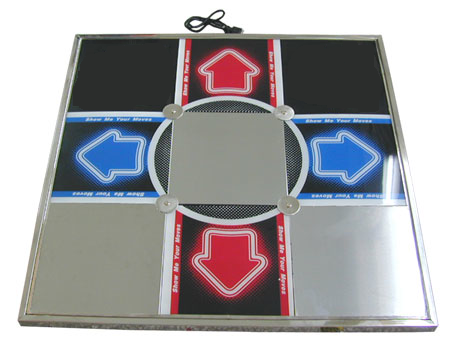
\includegraphics[width=0.4\textwidth]{dansmatta.png}
\caption{En dansmatta.}
\end{figure}

Johan hoppar runt på sin dansmatta nästan varje dag, men tycker det är svårt att hinna flytta sina fötter ibland. Därför vill han ha hjälp med att spela en låt så optimalt som möjligt - här innebär det alltså att flytta sina fötter så få gånger som möjligt.

I början har Johan sin ena fot på den vänstra pilen, och sin andra fot på den högra.

Givet en låt och vilka \emph{en eller två} pilar som måste vara nedtryckta i varje takt, beräkna det minsta antalet förflyttningar som Johan måste göra för att träffa alla pilar. Att byta plats på båda fötterna i ett hopp räknas som två förflyttningar.


\section*{Indata}
Den första raden består av det positiva heltalet $1 \le N \le 10\,000$, antal takter i låten.

Sedan följer $N$ rader, en rad för varje takt. Varje rad består av en sträng med \emph{en eller två} bokstäver som är några av \texttt{U}, \texttt{H}, \texttt{N} eller \texttt{V} för "upp", "höger", "ner", "vänster", respektive. Dessa är pilarna som måste vara nedtryckta under takten.

\section*{Utdata}
Den första och enda raden ska bestå av ett heltal $F$, det minsta antalet förflyttningar Johan måste göra.

\section*{Exempel}
I det första exempelfallet börjar Johan med fötterna på höger och vänster platta (som alltid). Sedan kan en optimal lösning t.ex. se ut som följer: Johan väljer att flytta höger fot till \texttt{U}-pilen, för att uppfylla det första kravet. Sedan flyttar han samma fot igen, den här gången till \texttt{N}-pilen. Johan står sedan still de kommande två takterna som kräver \texttt{V}-pilen nedtryckt (han står kvar där med vänsterfoten), och flyttar sedan någon av fötterna till \texttt{H}-pilen. Svaret är alltså 3 förflyttningar.

\section*{Delpoäng}
I det här problemet kan du samla en del av poängen utan att lösa problemet fullständigt. För 20 poäng är det garanterat att $N$ är max 10, och Johan behöver bara trycka ner precis en fot per takt. För ytterligare 30 poäng behöver Johan bara trycka ner precis en fot per takt, men $N$ kan vara upp till $10\,000$. För resterande 50 poäng måste ditt program klara att en eller två fötter måste vara nedtryckta per takt, och $N$ kan vara max $10\,000$.
